\chapter{Quotient Spaces}

Let $S$ be a subspace of a vector space $V$. Recalling the modular arithmetic, it is easy to see that the binary relation on $V$ defined binary
\[
	u \equiv v \iff u-v \in S
\]
is an equivalence relation. We say that $u$ and $v$ are \textbf{congruent modulo $S$}.

Now notice that
\begin{equation*}
	\begin{aligned}
		[v] &= \{ u \in V : u \equiv v \} \\
			&= \{ u \in V : u-v \in S \} \\
			&= \{ u \in V : u = v+s, \text{ for some } s \in S \} \\
			&= \{ v + s : s \in S \} \\
			&= v + S
	\end{aligned}
\end{equation*}

The set
\[
	[v] = v + S = \{ v+s : s \in S \}
\]
is called a \textbf{coset} or \textbf{affine subset} of $S$ in $V$.

\begin{example}
	The solution set of a linear system 
	\[
		C = \{ x : Ax = b \}
	\]
	is an affine subspace, with $A \in \mathbb{R}^{m \times n}$ and $b \in \mathbb{R}^m$.
\end{example}

\begin{definition}[Quotient Space]
	The set of all cosets (or classes) of $S$ in $V$, denoted by
\[
	V / S = \{ v+s : v \in V \}
\]
is called the \textbf{quotient space of $V$ modulo $S$}.
\end{definition}

Naturally, we define addition and scalar multiplication as follows
\[
	(u + S) + (v + S) = (u + v) + S \text{ and } \lambda(u+S) = \lambda u + S
\]
which are well defined.

\begin{theorem}
	The quotient space of $V$ modulo $S$ is a vector space over $\mathbb{F}$ with the operations
	\[
		\lambda(u + S) = \lambda u + S
	\]
	\[
		(u + S) + (v + S) = (u + v) + S
	\]
\end{theorem}

\begin{definition}[Natural Projection]
	If $S$ is a subspace of $V$, we may define the mapping 
	\begin{equation*}
		\begin{aligned}
			\pi_S : V &\longrightarrow V/S \\
			v &\longmapsto [v]
		\end{aligned}
	\end{equation*}
	which sends every vector to the coset containing it, i.e., the class associated to it. This map is called the \textbf{natural projection} or \textbf{canonical projection}.
\end{definition}

\begin{theorem}
	The canonical projection $\pi_S$ is a surjective linear mapping with $\ker (\pi_S) = S$.
\end{theorem}

\begin{theorem}[The Correspondence Theorem]
	Let $S$ be a subspace of $V$. Then the function that assigns each subspace $S \subset T \subset V$, the subspace $T/S$ of $V/S$ is an order-preserving one-to-one correspondence between the set of all subspaces of $V$ containing $S$ and the set of all subspaces of $V/S$.
\end{theorem}

\begin{figure}[h]
	\centering
	  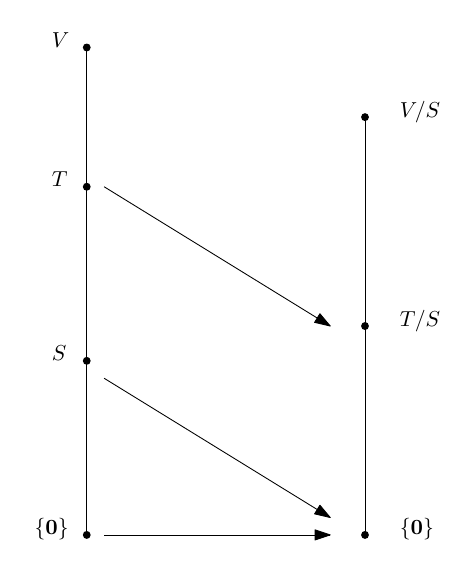
\includegraphics[width=0.37\textwidth]{Figures/correspondence_theorem.png} 
	  \caption{Correspondence between $V$ and $V/S$.}
	  \label{fig:correspondence-theorem}
\end{figure}

\begin{theorem}[Universal Property of Quotient]
	Let $V, U$ vector spaces over $\mathbb{F}$ and $T \in \hom(V, U)$. If $W$ is a subspace of $V$ such that $W \subseteq \ker (T)$, then there exists a linear mapping 
	\[
		\tilde{T} : V / W \longrightarrow U
	\]
\end{theorem}

The `universal' here means that for all objects in the category, there is exactly one map from this object to $\mathfrak{1}$, i.e., the \textbf{terminal object}.

Note that $\ker (\tilde{T}) = 0_{V/\ker (T)}$. Then $\tilde{T}$ is injective and $\text{Im}(\tilde{T}) = \text{Im}(T)$. Hence,
\[
	V/\ker (T) \cong \text{Im}(T)
\]
which is the \textbf{First Theorem of Isomorphism}.

% https://q.uiver.app/?q=WzAsMyxbMCwwLCJWIl0sWzAsMiwiVi9cXGtlcihUKSJdLFsyLDAsIlQoVikiXSxbMCwyLCJUIl0sWzAsMSwiXFx2YXJwaGkiLDJdLFsxLDIsIlxcY29uZyIsMix7InN0eWxlIjp7ImJvZHkiOnsibmFtZSI6ImRhc2hlZCJ9fX1dXQ==
\[\begin{tikzcd}
	V && {T(V)} \\
	\\
	{V/\ker(T)}
	\arrow["T", from=1-1, to=1-3]
	\arrow["\varphi"', from=1-1, to=3-1]
	\arrow["\cong"', dashed, from=3-1, to=1-3]
\end{tikzcd}\]

\begin{definition}[Codimension]
	Let $W$ be a subspace of $V$. Then the \textbf{codimension} of $W$ in $V$ is
	\[
		\text{codim}_V W = \dim V/W
	\]
\end{definition}

\begin{theorem}
	Suppose $\dim V = n$ and $W$ is a subspace of $V$ with $\dim W = k$. Then 
	\[
		\dim V/W = \text{codim}_V W = n-k
	\]
\end{theorem}

\begin{definition}[Cokernel and Coimage]
	Let $T : V \longrightarrow W$ a linear transformation. Then the \textbf{cokernel} of $T$ is the quotient space
	\[
		\text{coker} (T) = W / \text{Im}(T)
	\] 

	And the \textbf{coimage} of $T$ is defined as
	\[
		\text{coim} (T) = V / \text{Ker}(T)
	\]
\end{definition}

\begin{corollary}
	Let $V$ be a finite-dimensional vector space $T : V \longrightarrow V$ a linear transformation. Then 
	\[
		\dim (\ker (T)) = \dim (\text{coker} (T))
	\]
\end{corollary}